\documentclass{oblivoir}

\setmainfont{Fira Sans}
\setmainhangulfont[BoldFont={* Bold}]{KoPubWorld Dotum.ttf}

\usepackage{tikz}
\usetikzlibrary{shapes,arrows}

% Define block styles
\tikzstyle{decision} = [diamond, draw, fill=blue!20,
    text width=4.5em, text badly centered, node distance=3cm, inner sep=0pt]
\tikzstyle{block} = [rectangle, draw, fill=white!20,
    text width=10em, text badly centered, rounded corners, minimum height=2em]
\tikzstyle{line} = [draw, -latex']

\begin{document}
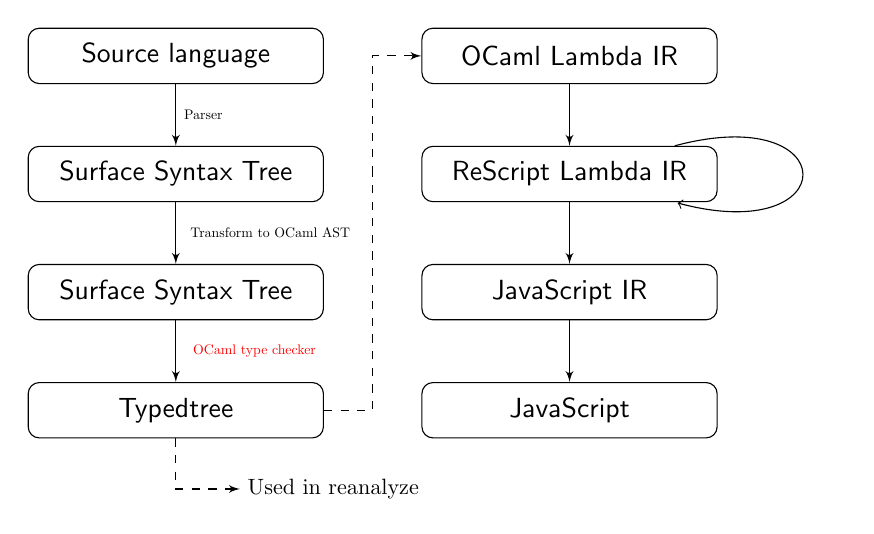
\begin{tikzpicture}[node distance = 1.5cm]
  % Place nodes
  \node [block] (src) {\textsf{Source language}};
  \node [block, below of=src] (ast1) {\textsf{Surface Syntax Tree}};
  \node [coordinate, right of=ast1, xshift=1cm] (temp){};
  \node [block, below of=ast1] (ast2) {\textsf{Surface Syntax Tree}};
  % Draw edges
  \path [line] (src) -- (ast1);
  \path [line] (ast1) -- (ast2);
  % Comments
  \node [below of=src, xshift=0.35cm, yshift=0.75cm, scale=0.5] (c1) {Parser};
  \node [below of=ast1, xshift=1.2cm, yshift=0.75cm, scale=0.5] (c2) {Transform to OCaml AST};

  % Place nodes
  \node [block, below of=ast2] (tast) {\textsf{Typedtree}};
  % Draw edges
  \path [line] (ast2) -- (tast);
  % Comment
  \node [below of=ast2, xshift=1cm, yshift=0.75cm, scale=0.5] (c3) {\color{red}OCaml type checker};

  % Place nodes
  \node [block, right of=src, xshift=3.5cm] (lam1) {\textsf{OCaml Lambda IR}};
  \node [block, below of=lam1] (lam2) {\textsf{ReScript Lambda IR}};
  % Draw edges
  \node [block, below of=lam2] (lam3) {\textsf{JavaScript IR}};
  \node [block, below of=lam3] (js) {\textsf{JavaScript}};
  \draw [-,dashed] (tast) -| (temp);
  \path [line,dashed] (temp) |- (lam1);
  \path [line] (lam1) -- (lam2);
  \path [line] (lam2) -- (lam3);
  \path [line] (lam3) -- (js);
  \path (lam2) edge [loop right] node {} (lam2);

  % Place nodes
  \node [below of=tast, yshift=0.5cm, xshift=2cm, scale=0.8] (c4) {Used in reanalyze};
  % Draw edges
  \path [line,dashed] (tast) |- (c4);
\end{tikzpicture}
\end{document}
%%% Local Variables: 
%%% coding: utf-8
%%% mode: latex
%%% TeX-engine: xetex
%%% End:
